% Options for packages loaded elsewhere
\PassOptionsToPackage{unicode}{hyperref}
\PassOptionsToPackage{hyphens}{url}
\documentclass[
  11pt,
]{article}
\usepackage{xcolor}
\usepackage[margin=0.75in]{geometry}
\usepackage{amsmath,amssymb}
\setcounter{secnumdepth}{-\maxdimen} % remove section numbering
\usepackage{iftex}
\ifPDFTeX
  \usepackage[T1]{fontenc}
  \usepackage[utf8]{inputenc}
  \usepackage{textcomp} % provide euro and other symbols
\else % if luatex or xetex
  \usepackage{unicode-math} % this also loads fontspec
  \defaultfontfeatures{Scale=MatchLowercase}
  \defaultfontfeatures[\rmfamily]{Ligatures=TeX,Scale=1}
\fi
\usepackage{lmodern}
\ifPDFTeX\else
  % xetex/luatex font selection
\fi
% Use upquote if available, for straight quotes in verbatim environments
\IfFileExists{upquote.sty}{\usepackage{upquote}}{}
\IfFileExists{microtype.sty}{% use microtype if available
  \usepackage[]{microtype}
  \UseMicrotypeSet[protrusion]{basicmath} % disable protrusion for tt fonts
}{}
\makeatletter
\@ifundefined{KOMAClassName}{% if non-KOMA class
  \IfFileExists{parskip.sty}{%
    \usepackage{parskip}
  }{% else
    \setlength{\parindent}{0pt}
    \setlength{\parskip}{6pt plus 2pt minus 1pt}}
}{% if KOMA class
  \KOMAoptions{parskip=half}}
\makeatother
\usepackage{color}
\usepackage{fancyvrb}
\newcommand{\VerbBar}{|}
\newcommand{\VERB}{\Verb[commandchars=\\\{\}]}
\DefineVerbatimEnvironment{Highlighting}{Verbatim}{commandchars=\\\{\}}
% Add ',fontsize=\small' for more characters per line
\newenvironment{Shaded}{}{}
\newcommand{\AlertTok}[1]{\textcolor[rgb]{1.00,0.00,0.00}{\textbf{#1}}}
\newcommand{\AnnotationTok}[1]{\textcolor[rgb]{0.38,0.63,0.69}{\textbf{\textit{#1}}}}
\newcommand{\AttributeTok}[1]{\textcolor[rgb]{0.49,0.56,0.16}{#1}}
\newcommand{\BaseNTok}[1]{\textcolor[rgb]{0.25,0.63,0.44}{#1}}
\newcommand{\BuiltInTok}[1]{\textcolor[rgb]{0.00,0.50,0.00}{#1}}
\newcommand{\CharTok}[1]{\textcolor[rgb]{0.25,0.44,0.63}{#1}}
\newcommand{\CommentTok}[1]{\textcolor[rgb]{0.38,0.63,0.69}{\textit{#1}}}
\newcommand{\CommentVarTok}[1]{\textcolor[rgb]{0.38,0.63,0.69}{\textbf{\textit{#1}}}}
\newcommand{\ConstantTok}[1]{\textcolor[rgb]{0.53,0.00,0.00}{#1}}
\newcommand{\ControlFlowTok}[1]{\textcolor[rgb]{0.00,0.44,0.13}{\textbf{#1}}}
\newcommand{\DataTypeTok}[1]{\textcolor[rgb]{0.56,0.13,0.00}{#1}}
\newcommand{\DecValTok}[1]{\textcolor[rgb]{0.25,0.63,0.44}{#1}}
\newcommand{\DocumentationTok}[1]{\textcolor[rgb]{0.73,0.13,0.13}{\textit{#1}}}
\newcommand{\ErrorTok}[1]{\textcolor[rgb]{1.00,0.00,0.00}{\textbf{#1}}}
\newcommand{\ExtensionTok}[1]{#1}
\newcommand{\FloatTok}[1]{\textcolor[rgb]{0.25,0.63,0.44}{#1}}
\newcommand{\FunctionTok}[1]{\textcolor[rgb]{0.02,0.16,0.49}{#1}}
\newcommand{\ImportTok}[1]{\textcolor[rgb]{0.00,0.50,0.00}{\textbf{#1}}}
\newcommand{\InformationTok}[1]{\textcolor[rgb]{0.38,0.63,0.69}{\textbf{\textit{#1}}}}
\newcommand{\KeywordTok}[1]{\textcolor[rgb]{0.00,0.44,0.13}{\textbf{#1}}}
\newcommand{\NormalTok}[1]{#1}
\newcommand{\OperatorTok}[1]{\textcolor[rgb]{0.40,0.40,0.40}{#1}}
\newcommand{\OtherTok}[1]{\textcolor[rgb]{0.00,0.44,0.13}{#1}}
\newcommand{\PreprocessorTok}[1]{\textcolor[rgb]{0.74,0.48,0.00}{#1}}
\newcommand{\RegionMarkerTok}[1]{#1}
\newcommand{\SpecialCharTok}[1]{\textcolor[rgb]{0.25,0.44,0.63}{#1}}
\newcommand{\SpecialStringTok}[1]{\textcolor[rgb]{0.73,0.40,0.53}{#1}}
\newcommand{\StringTok}[1]{\textcolor[rgb]{0.25,0.44,0.63}{#1}}
\newcommand{\VariableTok}[1]{\textcolor[rgb]{0.10,0.09,0.49}{#1}}
\newcommand{\VerbatimStringTok}[1]{\textcolor[rgb]{0.25,0.44,0.63}{#1}}
\newcommand{\WarningTok}[1]{\textcolor[rgb]{0.38,0.63,0.69}{\textbf{\textit{#1}}}}
\usepackage{longtable,booktabs,array}
\newcounter{none} % for unnumbered tables
\usepackage{calc} % for calculating minipage widths
% Correct order of tables after \paragraph or \subparagraph
\usepackage{etoolbox}
\makeatletter
\patchcmd\longtable{\par}{\if@noskipsec\mbox{}\fi\par}{}{}
\makeatother
% Allow footnotes in longtable head/foot
\IfFileExists{footnotehyper.sty}{\usepackage{footnotehyper}}{\usepackage{footnote}}
\makesavenoteenv{longtable}
\usepackage{graphicx}
\makeatletter
\newsavebox\pandoc@box
\newcommand*\pandocbounded[1]{% scales image to fit in text height/width
  \sbox\pandoc@box{#1}%
  \Gscale@div\@tempa{\textheight}{\dimexpr\ht\pandoc@box+\dp\pandoc@box\relax}%
  \Gscale@div\@tempb{\linewidth}{\wd\pandoc@box}%
  \ifdim\@tempb\p@<\@tempa\p@\let\@tempa\@tempb\fi% select the smaller of both
  \ifdim\@tempa\p@<\p@\scalebox{\@tempa}{\usebox\pandoc@box}%
  \else\usebox{\pandoc@box}%
  \fi%
}
% Set default figure placement to htbp
\def\fps@figure{htbp}
\makeatother
\setlength{\emergencystretch}{3em} % prevent overfull lines
\providecommand{\tightlist}{%
  \setlength{\itemsep}{0pt}\setlength{\parskip}{0pt}}
\usepackage{bookmark}
\IfFileExists{xurl.sty}{\usepackage{xurl}}{} % add URL line breaks if available
\urlstyle{same}
\hypersetup{
  pdftitle={Balanced Hidden-Spin Feedback for Prime-Sequence Fidelity Through One Billion},
  pdfauthor={Sean Brady --- Originator and Conceptual Director},
  hidelinks,
  pdfcreator={LaTeX via pandoc}}

\title{Balanced Hidden-Spin Feedback for Prime-Sequence Fidelity Through
One Billion}
\author{Sean Brady --- Originator and Conceptual Director}
\date{27 September 2026 · Zenodo companion paper, version 1.1}

\usepackage{fvextra,seqsplit,needspace}
\DefineVerbatimEnvironment{Highlighting}{Verbatim}{commandchars=\\\{\},breaklines,fontsize=\footnotesize}
\AtBeginEnvironment{longtable}{\footnotesize}
\begin{document}
\maketitle

\textbf{AI research collaborators:} OpenAI ChatGPT and Codex.

\textbf{SAM Research Project.} Computational research paper; numerical
results are drawn from completed, retained experiments.

\textbf{Software concept DOI:}
\url{https://doi.org/10.5281/zenodo.23002148}\\
\textbf{Initial archived software version (0.1.0):}
\url{https://doi.org/10.5281/zenodo.23002149}\\
\textbf{Repository:} \url{https://github.com/iwtbotiwtwot/prime-event}\\
\textbf{Paper license:} CC BY 4.0. \textbf{Software license:} MIT.

This paper accompanies the software release. The identifiers above
identify the software archive; this document does not assign itself a
separate publication DOI.

\section{Abstract}\label{abstract}

Stochastic logic used inside a recurrence system can produce rare local
errors that alter its subsequent input history. We investigate this
problem using a seven-spin heat-bath model coupled to an event-created
digital sieve. Each accepted integer installs a periodic return channel,
and two banks aggregate those returns into the inputs of a gate with one
output spin and six hidden spins. Acceptance requires three successive
output readings. In an initial ensemble of 64 pseudorandom seeds under
each of two matched-exposure accumulation profiles, one seed per profile
reproduces every prime and rejects every composite through \(10^9\).
Microscopic replay locates all 120 first composite emissions in the
single-return-bank sector. Integrating out the hidden spins gives the
output field \(H=-a(r_1+r_2)+br_1r_2\), whose two blocking margins are
\(b\) and \(2a-b\). Equalizing these margins selects \(b=a\)
algebraically, before the successor trajectories are generated. With the
same cadence, random streams, confirmation rule, and recurrence
scheduler, the balanced source raises the number of exact trajectories
from 1/64 to 47/64 per profile and reduces the aggregate error count
from 569 to 40 across the paired profiles, a 92.97\% reduction. A
frozen-source continuation on 16 fresh seed pairs yields 13/16 exact
trajectories per profile through \(10^9\). The study connects
microscopic error diagnosis, effective-interaction design, and
long-horizon sequence fidelity in a stochastic feedback computation.
Exactness denotes complete agreement of specified finite trajectories
with an independent reference sieve. The recurrence arithmetic is
supplied by the digital scheduler; the measured contribution is the
reliability improvement obtained by balancing the hidden-spin gate.

\textbf{Keywords:} stochastic spin logic; hidden spins; effective
interactions; prime sieve; recurrence; rare-event errors; feedback;
reproducible computation.

\section{1. Introduction}\label{introduction}

A stochastic gate can be locally accurate yet accumulate appreciable
sequence error over a billion decisions. When accepted outputs change
the future inputs, its errors also become part of the computation's
evolving history. The relevant object is therefore the entire coupled
trajectory: its microscopic state, sampled readings, accepted events,
and the future constraints created by those events.

Prime enumeration supplies a sharply defined setting for studying this
behavior. Starting at integer 2, an accepted integer can install a
channel that returns at its positive multiples beginning with twice its
value. An ideal gate accepts precisely when no earlier channel returns.
The resulting recurrence enumerates the primes. Replacing that ideal
decision with a finite stochastic spin gate creates an explicit
question: how faithfully does the coupled system preserve this sequence,
and can a diagnosed microscopic weakness be corrected through its
interaction terms?

Probabilistic spin logic provides an established context for such a
question. Camsari, Sutton, and Datta describe p-bits and circuit
representations for stochastic computation {[}1{]}. Arithmetic sieving
also has physical and unconventional-computing precedents. Petersen and
colleagues encode prime sieves in wave superpositions and diffraction
{[}2{]}, while Monaco and Vindiola use neuromorphic computation for the
smoothness-sieving stage of integer factorization {[}3{]}. A public
rotating-circle implementation describes the closely related idea of
adding a new oscillator when no existing oscillator returns at an
integer tick {[}4{]}. These precedents motivate a specific contribution
here: the diagnosis and algebraic repair of a stochastic hidden-spin
readout embedded in an event-created recurrence network.

The experiment originated in studies of unequal tick durations and
accumulation-dependent spin response. Those studies supplied a common
geometric cadence and two accumulation profiles. The present manuscript
concentrates on the prime-feedback experiment, whose completed record
supports three linked results. First, replay transfers every tested
first error with its three random readings. Second, the observed
vulnerable input sector is exactly the sector in which the gate's pair
contributions cancel. Third, equalizing the remaining blocking margins
substantially improves billion-index fidelity, including on fresh random
streams.

\section{2. Model and numerical
methods}\label{model-and-numerical-methods}

\subsection{2.1 Event-created recurrence and bank
inputs}\label{event-created-recurrence-and-bank-inputs}

Let \(n=2,3,\ldots,N\) be the candidate index, with \(N=10^9\).
Initially there are no channels. If candidate \(p\) is accepted, it
creates a channel returning at \(2p,3p,\ldots\). Channels are assigned
alternately to banks 0 and 1 according to their creation order, starting
with bank 0. For each candidate, the input \(r_i\in\{-1,+1\}\) records
absence or presence of a return in bank \(i\). Multiple simultaneous
returns in the same bank produce the same input as one return.

With an ideal gate, a candidate is accepted exactly when both inputs are
\(-1\). At a prime, no earlier accepted prime divides the candidate and
there is no return. At a composite, an earlier prime divisor supplies a
return. This establishes the connection between the supplied recurrence
rule and the target sequence by induction from candidate 2.

The stochastic implementation retains this scheduler but replaces the
ideal decision with three spin readings. A false emission installs an
additional channel; a missed prime omits a channel. Either can alter
subsequent inputs. In addition, an extra or missing event changes the
parity of the creation count and therefore changes the bank assignment
of subsequent channels.

The production scheduler uses a horizon-length byte array to store the
two bank bits. On acceptance of \(n\), it marks the appropriate bit at
every multiple from \(2n\) through \(N\). This is a digital sieve
implementation. Generation uses no external prime labels, but the
divisibility structure is explicitly encoded by these integer-multiple
updates. The reported experiment is a CPU simulation of the coupled
scheduler and spin model.

\subsection{2.2 Microscopic energy and effective output
field}\label{microscopic-energy-and-effective-output-field}

There are seven dynamic spins: output \(e\in\{-1,+1\}\) and hidden spins
\(h_1,\ldots,h_6\in\{-1,+1\}\). The two bank inputs are clamped during a
candidate's three readings. At dimensionless inverse temperature
\(\beta=1\), write \(x=(e,r_1,r_2)^T\) and

\[
E(e,\mathbf h\mid r_1,r_2)=-\sum_{j=1}^{6}h_j[(Wx)_j+\eta_j]. \tag{1}
\]

The complete source is

\[
W=\begin{pmatrix}
4&4&0\\4&0&4\\-t&-t&t\\-t&t&-t\\t&-t&-t\\t&t&t
\end{pmatrix},\qquad
\boldsymbol\eta=(0,0,t,t,t,t)^T. \tag{2}
\]

The first two rows are pair modules; the final four rows form the triple
module. Hidden spins are conditionally independent at fixed
\(e,r_1,r_2\), so summing over them gives

\[
F(e\mid r_1,r_2)=-\sum_{j=1}^{6}\log[2\cosh((Wx)_j+\eta_j)]
=C(r_1,r_2)+eH(r_1,r_2), \tag{3}
\]

where the output-independent term \(C\) need not be evaluated for the
readout, and

\[
H=-a(r_1+r_2)+br_1r_2,\qquad
a=\tfrac12\log\cosh8,\qquad
b(t)=\tfrac12\log\frac{\cosh^4(2t)}{\cosh4t}. \tag{4}
\]

The accepted output is \(e=-1\). Its conditional equilibrium probability
is

\[
P_{\mathrm{eq}}(e=-1\mid r_1,r_2)=\frac{1}{1+\exp(-2H)}. \tag{5}
\]

No-return inputs give \(H=2a+b>0\), favoring acceptance. One returning
bank gives \(H=-b\) because the pair terms cancel. Two returning banks
give \(H=b-2a\). Thus the two blocking margins are \(b\) and \(2a-b\).

\subsection{2.3 State dynamics and temporal
confirmation}\label{state-dynamics-and-temporal-confirmation}

We enumerate all \(2^7=128\) microscopic states. Bit 0 encodes the
output, with even state indices representing \(e=-1\); the other six
bits encode the hidden spins. For states \(s\) and \(z\) differing by
one spin flip, the column-generator convention is

\[
(Q_0)_{z,s}=\frac{1}{1+\exp[E(z)-E(s)]},\qquad
(Q_0)_{s,s}=-\sum_{z\ne s}(Q_0)_{z,s}. \tag{6}
\]

Other off-diagonal entries are zero. All seven spins participate in
these heat-bath dynamics. The candidate's phase and accumulation profile
determine an exposure \(\tau_k\); each of its three readings uses

\[
T_{k,r_1,r_2}=\exp(Q_0\Gamma\tau_k/3),\qquad \Gamma=512. \tag{7}
\]

Each sampled state becomes the initial state for the next reading. The
final state is carried into the next candidate. All three readings are
taken even if an earlier reading rejects the candidate. A candidate is
accepted only if all three sampled output spins equal \(-1\).

Let \(D\) be the diagonal mask selecting even states. For incoming state
vector \(v_s\), the exact finite-state expression for acceptance is

\[
P_{\mathrm{accept}}(s)=\mathbf{1}^TDTDTDTv_s. \tag{8}
\]

The expression retains correlations between readings and is evaluated
numerically. It is not replaced in the simulation by the cube of an
equilibrium probability. The trajectory begins with a sample from the
no-return Gibbs distribution of its own source.

\subsection{2.4 Unequal geometric ticks and matched accumulation
exposure}\label{unequal-geometric-ticks-and-matched-accumulation-exposure}

Both profiles inherit a 35-step geometric duration sequence \(d_k\) from
a retained corrugated-surface construction with circulation counts 5 and
7. The duration values have mean one and range approximately from
0.963919 to 1.029631. The complete arrays are included with this
manuscript's evidence, permitting reproduction without reconstructing
the geometric precursor.

Uniform accumulation uses \(A_k=1/4\). Rough accumulation uses

\[
A_k=\frac14+0.1\cos\left(\frac{2\pi5(k+1/2)}{35}+\frac\pi7\right)
+0.05\sin\left(\frac{2\pi11(k+1/2)}{35}\right),\quad k=0,\ldots,34. \tag{9}
\]

For each profile,

\[
\tau_k=c\,d_k\sqrt{1-A_k},\qquad
c=\frac{\sqrt{3/4}\sum_kd_k}{\sum_kd_k\sqrt{1-A_k}}. \tag{10}
\]

This normalizes total exposure over a 35-step cycle. The rough
normalization factor is approximately 1.001445056101028; the uniform
factor is one up to floating-point rounding. Candidate \(n\) uses phase
\(k=(n-2)\bmod35\). ``Uniform'' refers to accumulation, not to geometric
tick duration. The accumulation-to-rate mapping is a declared model
input; no measured physical clock calibration is used.

\subsection{2.5 Algebraic source
balancing}\label{algebraic-source-balancing}

The baseline uses \(t=2\), giving \(a=3.6534264659876117\) and
\(b=2.9609499856382886\). Its one-bank blocking margin is weaker than
its two-bank margin. At fixed \(a>0\),

\[
\min(b,2a-b)\le a, \tag{11}
\]

with equality at \(b=a\). This maximum-minimum criterion selected the
successor source before its event outputs were examined. It equalizes
the blocking margins; it does not assert an optimum of total trajectory
errors, which also depend on input frequencies and dynamics.

For a closed-form specification, set \(C=\cosh8\) and \(z=\cosh^2(2t)\).
The equation \(b(t)=a\) gives \(z^2=C(2z-1)\). The admissible root
yields

\[
t_* = \frac12\operatorname{acosh}\sqrt{C+\sqrt{C^2-C}}
\simeq2.3464897298984759. \tag{12}
\]

The native source builder solves the same equation numerically. Pair
strength remains 4; the four triple rows and their fields increase
together by approximately 17.3\%. The topology, temperature, cadence,
and readout count remain fixed. The total coupling-strength budget
increases. This is a fixed-temperature construction, distinct from
separate all-temperature ratio-locking studies.

\subsection{2.6 Seeds, matching, and
scoring}\label{seeds-matching-and-scoring}

The matched campaign includes every seed from 1000000 through 1000063,
under both profiles. The baseline is the frozen billion-index
predecessor, with no baseline rerun. The balanced campaign uses the same
seed assignments, chunking, cadence, scheduler, and sampling convention.
Its two profiles share each seed's random streams, making this 64 paired
seed cases rather than 128 independent replications.

NumPy PCG64 supplies a base stream seeded with \(s\) and an auxiliary
stream seeded with \(s+1000000\). The base stream first samples the
initial state, then supplies the third reading for each candidate. The
auxiliary stream supplies the first two readings. The incoming state's
transition CDF is searched for the first entry strictly greater than the
random draw. Five-million-candidate chunks preserve the generator states
and ending microscopic state.

After the matched experiment, a frozen-source continuation includes all
16 seeds from 10000000 through 10000015 under both profiles. Neither
source retuning nor seed screening occurs. Base and auxiliary seed
ranges are disjoint from the matched experiment. These are fresh-stream
observations; there is no corresponding fresh-seed baseline ensemble.

An independent prime sieve scores every emitted bit after generation. A
false positive (FP) is an emitted composite; a false negative (FN) is a
missed prime. An exact trajectory has FP=FN=0 over every integer from 2
through its stated horizon. At \(10^9\), an exact trajectory contains
50,847,534 emitted primes. Exactness here is a property of a completed
finite realization; source probabilities and propagators are represented
in binary64 arithmetic.

\section{3. Results}\label{results}

\subsection{3.1 Microscopic replay identifies the vulnerable
sector}\label{microscopic-replay-identifies-the-vulnerable-sector}

In the baseline, only seed 1000063 is exact through \(10^9\) under both
profiles. All baseline seeds have the same source parameters and
initially sample state 56. The mechanism study compares each of the 63
failing seeds with seed 1000063 at its first error under each profile,
giving 126 local comparisons. Before a first error, the two trajectories
have emitted the same events and therefore have the same bank inputs.

Exchanging the three draws while retaining the failing seed's incoming
state corrects all 126 decisions. Exchanging the incoming state while
retaining the failing draws leaves all 126 decisions incorrect. In 32
comparisons the incoming states were already identical. The observed
discriminator is the realized random triple, rather than a protective
incoming state associated with seed 1000063.

Of the 126 first errors, 120 are composite emissions and six are missed
primes. Every first composite emission occurs with exactly one returning
bank. This is the sector in which Eq. (4)'s pair contributions cancel.
The baseline three-reading false-emission probability is approximately
\(1.91\times10^{-8}\) for one-bank input, compared with approximately
\(4.74\times10^{-12}\) for two-bank input. The opportunity counts
differ, so this ratio characterizes local susceptibility rather than the
ratio of total errors.

One replay exposes the microscopic decision directly. At prime
3,510,937, seed 1000002 and seed 1000063 both enter in state 103 with no
returns. The failing seed samples states \(56\to56\to101\); the exact
seed samples \(56\to56\to56\). The third failing draw falls in a
state-101 CDF interval only about \(3.77\times10^{-11}\) wide. Because
state 101 has rejecting output parity, that reading omits the prime.

The replay covers 230 selected chunks, totaling 1.15 billion decisions,
and retains 264 local windows. It reconstructs emitted bits, final
states, event counts, checksums, and RNG states. Its local interventions
diagnose the decision at a fixed history; they do not assume that the
entire later autonomous history remains unchanged after intervention.

\subsection{3.2 Balancing changes the three input
sectors}\label{balancing-changes-the-three-input-sectors}

Table 1 summarizes the algebraic change. The one-bank margin increases
while the stronger two-bank margin decreases to the same value. The
no-return field \(2a+b\) also increases, favoring correct acceptance.

\Needspace{9\baselineskip}
Table 1. Effective coefficients and blocking margins at \(\beta=1\).

{\def\LTcaptype{none} % do not increment counter
\begin{longtable}[]{@{}lrr@{}}
\toprule\noalign{}
Quantity & Baseline & Balanced \\
\midrule\noalign{}
\endhead
\bottomrule\noalign{}
\endlastfoot
Pair coefficient \(a\) & 3.653426466 & 3.653426466 \\
Triple coefficient \(b\) & 2.960949986 & 3.653426466 \\
One-bank margin \(b\) & 2.960949986 & 3.653426466 \\
Two-bank margin \(2a-b\) & 4.345902946 & 3.653426466 \\
Microscopic triple strength \(t\) & 2 & 2.346489730 \\
\end{longtable}
}

The full transition-matrix contractions decrease the one-bank
false-emission probability by approximately 60-fold. Across phases and
incoming states, the balanced uniform range is
\(3.021809\times10^{-10}\) to \(3.0442297\times10^{-10}\); the rough
range is \(3.0166175\times10^{-10}\) to \(3.0919287\times10^{-10}\). The
balanced two-bank probability is approximately \(3.014\times10^{-10}\).
Thus the source redistributes error susceptibility across the input
sectors, with the net outcome determined by the closed-loop experiment.

\begin{figure}
\centering
\pandocbounded{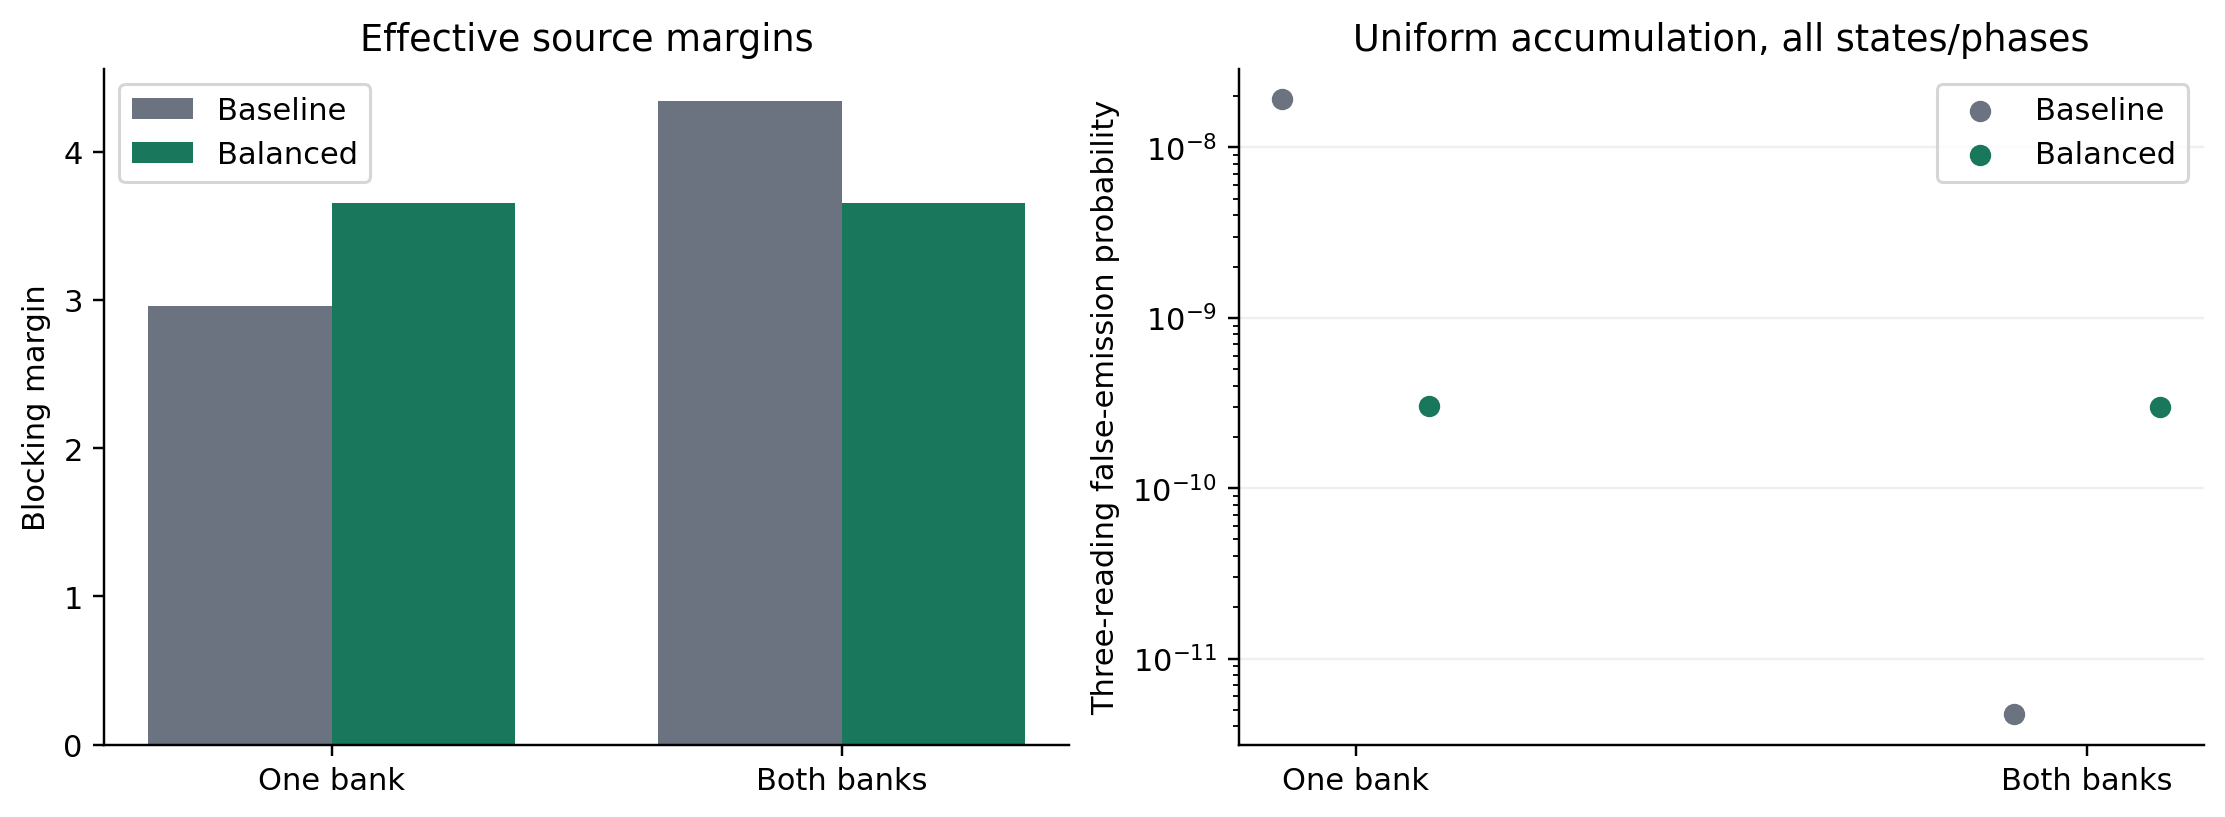
\includegraphics[keepaspectratio,alt={Blocking margins and full-state three-reading error probabilities. The probability ranges span all retained phases and incoming states; uniform-profile values are shown.}]{../manuscript/figures/source_balance.png}}
\caption{Blocking margins and full-state three-reading error
probabilities. The probability ranges span all retained phases and
incoming states; uniform-profile values are shown.}
\end{figure}

\subsection{3.3 Matched billion-index
trajectories}\label{matched-billion-index-trajectories}

All 128 balanced trajectories finish through \(10^9\). Table 2 reports
aggregate errors within each profile. The total across the two paired
profiles falls from 569 to 40, a 92.9701\% reduction. This is a
paired-profile descriptive total, not an independence-adjusted sample
size.

\Needspace{9\baselineskip}
Table 2. Matched seed outcomes through \(10^9\).

{\def\LTcaptype{none} % do not increment counter
\begin{longtable}[]{@{}
  >{\raggedright\arraybackslash}p{(\linewidth - 8\tabcolsep) * \real{0.1579}}
  >{\raggedleft\arraybackslash}p{(\linewidth - 8\tabcolsep) * \real{0.2105}}
  >{\raggedleft\arraybackslash}p{(\linewidth - 8\tabcolsep) * \real{0.2105}}
  >{\raggedleft\arraybackslash}p{(\linewidth - 8\tabcolsep) * \real{0.2105}}
  >{\raggedleft\arraybackslash}p{(\linewidth - 8\tabcolsep) * \real{0.2105}}@{}}
\toprule\noalign{}
\begin{minipage}[b]{\linewidth}\raggedright
Profile
\end{minipage} & \begin{minipage}[b]{\linewidth}\raggedleft
Baseline FP / FN
\end{minipage} & \begin{minipage}[b]{\linewidth}\raggedleft
Balanced FP / FN
\end{minipage} & \begin{minipage}[b]{\linewidth}\raggedleft
Exact: baseline → balanced
\end{minipage} & \begin{minipage}[b]{\linewidth}\raggedleft
Improved / equal / worse
\end{minipage} \\
\midrule\noalign{}
\endhead
\bottomrule\noalign{}
\endlastfoot
Uniform & 271 / 13 & 17 / 3 & 1/64 → 47/64 & 62 / 1 / 1 \\
Rough & 272 / 13 & 17 / 3 & 1/64 → 47/64 & 62 / 1 / 1 \\
\end{longtable}
}

The worst balanced trajectory has two errors. Seed 1000063 remains
exact, and the previously worst baseline seed 1000058 becomes exact. For
each profile, 62 seeds improve, one is unchanged, and one worsens. All
64 balanced uniform/rough pairs have identical emitted sequences,
although their transition matrices differ.

Exact-sequence counts make long-horizon fidelity visible without
allowing the many correctly rejected composites to dominate an overall
accuracy percentage. Table 3 gives the completed prefix comparisons.
Every matched balanced seed is exact through \(10^8\); by \(10^9\), 47
remain exact.

\Needspace{9\baselineskip}
Table 3. Number of exact matched trajectories out of 64, for each
profile.

{\def\LTcaptype{none} % do not increment counter
\begin{longtable}[]{@{}
  >{\raggedright\arraybackslash}p{(\linewidth - 8\tabcolsep) * \real{0.1579}}
  >{\raggedleft\arraybackslash}p{(\linewidth - 8\tabcolsep) * \real{0.2105}}
  >{\raggedleft\arraybackslash}p{(\linewidth - 8\tabcolsep) * \real{0.2105}}
  >{\raggedleft\arraybackslash}p{(\linewidth - 8\tabcolsep) * \real{0.2105}}
  >{\raggedleft\arraybackslash}p{(\linewidth - 8\tabcolsep) * \real{0.2105}}@{}}
\toprule\noalign{}
\begin{minipage}[b]{\linewidth}\raggedright
Horizon
\end{minipage} & \begin{minipage}[b]{\linewidth}\raggedleft
Uniform baseline
\end{minipage} & \begin{minipage}[b]{\linewidth}\raggedleft
Uniform balanced
\end{minipage} & \begin{minipage}[b]{\linewidth}\raggedleft
Rough baseline
\end{minipage} & \begin{minipage}[b]{\linewidth}\raggedleft
Rough balanced
\end{minipage} \\
\midrule\noalign{}
\endhead
\bottomrule\noalign{}
\endlastfoot
\(10^6\) & 64 & 64 & 64 & 64 \\
\(10^7\) & 60 & 64 & 60 & 64 \\
\(10^8\) & 42 & 64 & 42 & 64 \\
\(10^9\) & 1 & 47 & 1 & 47 \\
\end{longtable}
}

\begin{figure}
\centering
\pandocbounded{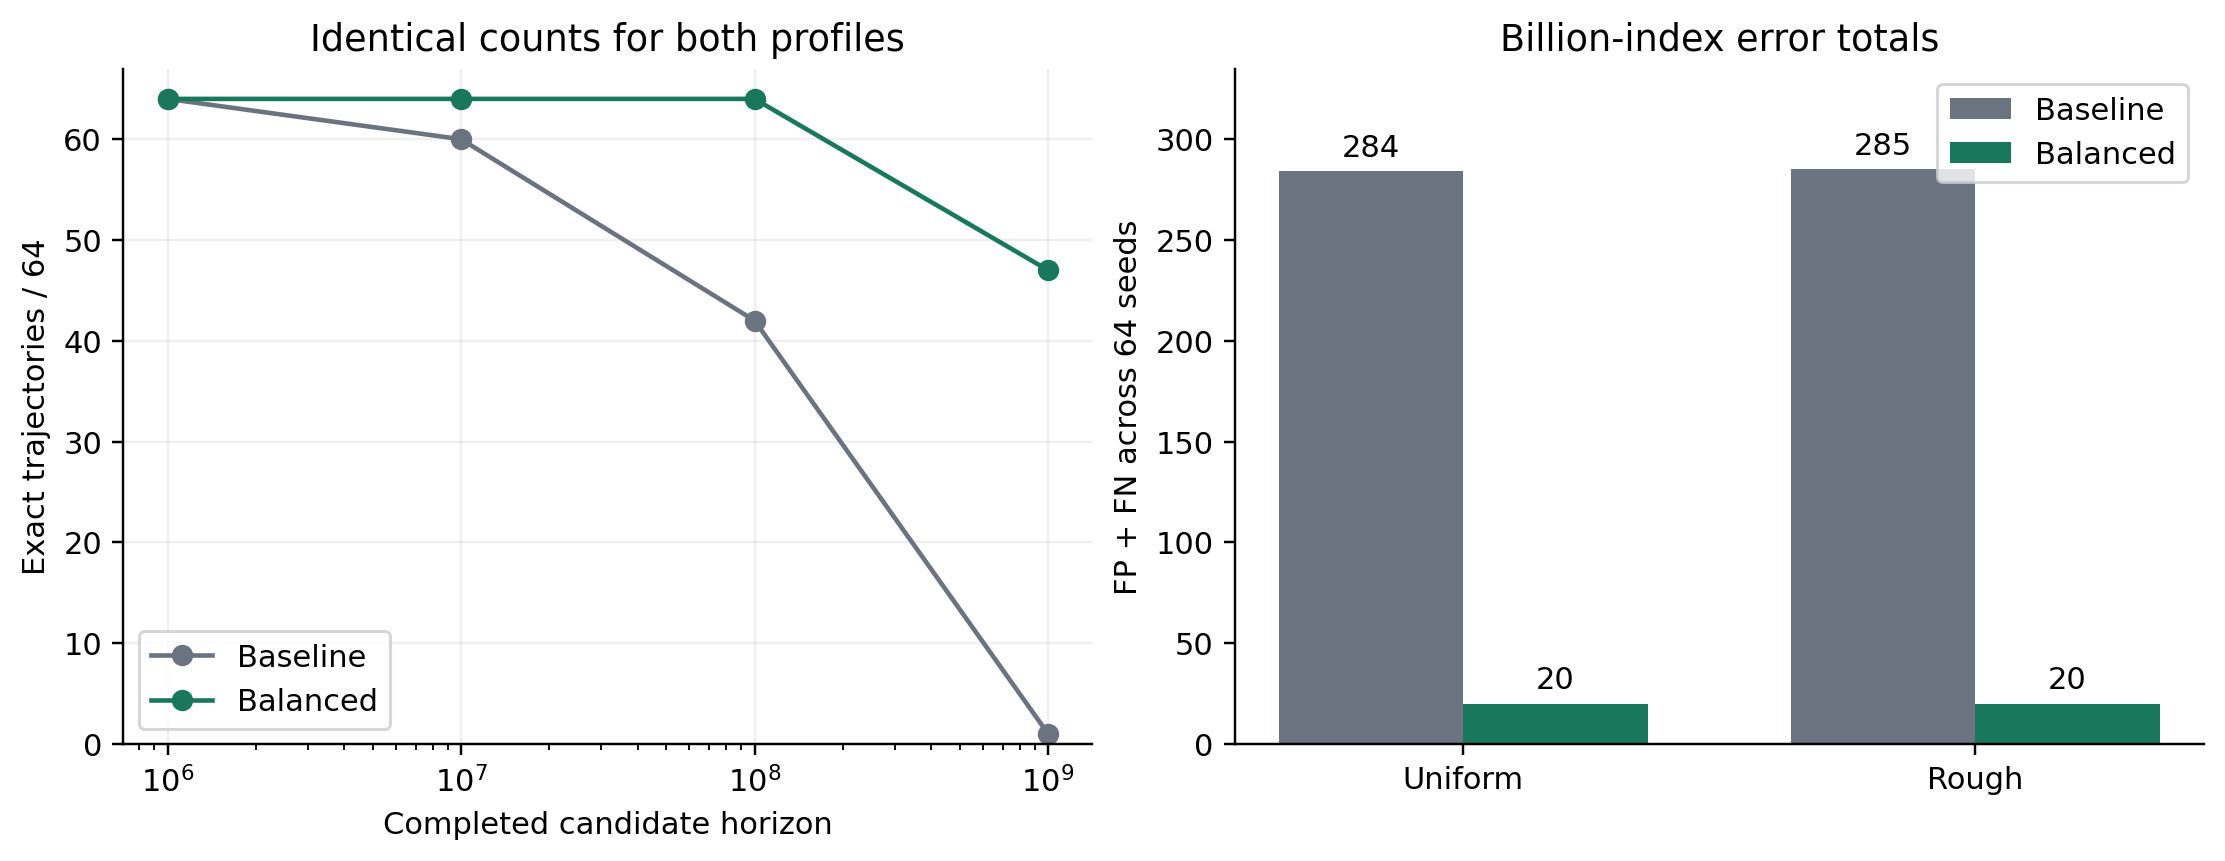
\includegraphics[keepaspectratio,alt={Matched-seed exact sequence counts and error totals. Both profiles are paired by seed; coincident survival curves have the same values.}]{../manuscript/figures/matched_results.png}}
\caption{Matched-seed exact sequence counts and error totals. Both
profiles are paired by seed; coincident survival curves have the same
values.}
\end{figure}

\subsection{3.4 Frozen-source fresh-seed
continuation}\label{frozen-source-fresh-seed-continuation}

All 32 fresh trajectories also finish through \(10^9\). In each profile,
13 of 16 are exact, with two composite emissions and one missed prime
across the ensemble. Fifteen of 16 are exact through \(10^8\). Each
failing trajectory has exactly one error. Uniform and rough outputs
agree within all 16 seed pairs.

\Needspace{9\baselineskip}
Table 4. Every fresh-seed error; the same three errors occur in both
profiles.

{\def\LTcaptype{none} % do not increment counter
\begin{longtable}[]{@{}lrl@{}}
\toprule\noalign{}
Seed & Candidate & Error \\
\midrule\noalign{}
\endhead
\bottomrule\noalign{}
\endlastfoot
10000012 & 82,866,449 & Composite emitted \\
10000004 & 203,033,716 & Composite emitted \\
10000006 & 997,044,317 & Prime omitted \\
\end{longtable}
}

The fresh-stream result extends the balanced source's observed
performance beyond the original seed roster. Its 13/16 count is reported
separately from the matched 47/64 count because the continuation has no
fresh baseline comparison and was conducted after the matched outcome
was known.

\subsection{3.5 An explicit feedback path from one event to later
inputs}\label{an-explicit-feedback-path-from-one-event-to-later-inputs}

The baseline contains an instructive profile-dependent chain. For seed
1000053, rough accumulation emits an extra composite at 312,596,611.
That additional event changes creation-count parity. When prime
483,920,363 is subsequently emitted, its channel is assigned to
different banks in the two profiles. At
\(967,840,726=2\times483,920,363\), its return coincides with the
period-2 channel. The uniform trajectory sees one returning bank and
emits the composite; the rough trajectory sees two returning banks and
rejects it.

The extra period 312,596,611 does not divide the later candidate. Its
effect is mediated by channel-assignment parity. This retained trace
demonstrates why local gate reliability and the recurrence history must
be analyzed together: an erroneous event can change later input
conditions without returning at the later index itself.

\section{4. Numerical verification and
reproducibility}\label{numerical-verification-and-reproducibility}

\subsection{4.1 Propagators and short-run
qualification}\label{propagators-and-short-run-qualification}

The source builder uses positive uniformization with scaling and
squaring, followed by column normalization, to compute the 128-state
propagators. It records series-tail estimates and normalization
adjustments. An independently implemented direct {[}13/13{]} Padé
exponential checks all 280 profile/phase/input matrices. After column
normalization, the largest matrix-entry difference is
\(1.5821\times10^{-14}\). The raw Padé drift and the initial
unnormalized comparison remain preserved with the source checks.

There are 1,080 source checks and 64,574 short-run qualification checks.
Short-run checks include scalar linear-CDF sampling, independently
reconstructed modulo-based returns, and ending state/count/checksum
agreement. These checks address numerical construction and
implementation agreement. They do not convert binary64 transition
probabilities into certified exact real-number probabilities.

\subsection{4.2 Complete output scoring and retained microscopic
evidence}\label{complete-output-scoring-and-retained-microscopic-evidence}

The matched campaign contains 25,600 checked chunks and 127,999,999,872
scored candidate decisions. The fresh continuation adds 6,400 checked
chunks and 31,999,999,968 decisions. Together, the balanced-source
phases contain 159,999,999,840 scored decisions. These counts include
paired profiles and repeated seed trajectories; they are not counts of
distinct integers.

Every emitted bit is scored against the independent reference sieve, and
chunk hashes and chains are checked. Retained microscopic prefixes
contribute 1,572,864 checked spin samples in the matched campaign and
393,216 in the continuation. Full microscopic state sequences were not
stored for every billion-index trajectory. Packed emissions, both bank
histories, RNG checkpoints, final states, running checksums, and source
arrays support targeted replay; the predecessor mechanism study performs
that replay on its selected chunks.

\subsection{4.3 Execution and storage}\label{execution-and-storage}

Source construction ran through source-bound ATOM3D/A3D41-T18-CONTACT-R2
on workstation SLC-GEN3-R4/CEV1-R4. Production used the retained
portable SLC-GEN4-P1/CE-P1 runtime with the operation
\texttt{\seqsplit{GEN4\_PRIME\_BALANCED\_CHUNKED}}. Source construction, short
qualification, matched production, and fresh production each retain
calculation, export, and checkpoint receipts: twelve successful native
calls in total. The portable GEN4 designation is a scoped runtime
identifier; this experiment introduced no global engine promotion.

Production used 28 workers on a pod with a 27.2-CPU quota and
approximately 466 GiB of RAM. Recorded CPU use was approximately 27.19
cores. Trajectories parallelize across seeds and profiles; within a
trajectory the candidate decisions are sequential because they update
both spin state and recurrence history. No GPU backend was used. Chunks
were packed and compressed in memory before disk flush and checkpoint
commit.

The matched archive contains 25,821,384,418 bytes; the fresh archive
contains 6,350,494,109 bytes. Both were transferred to the T500 and
verified against their manifests, for approximately 32.172 GB combined.
This manuscript presents no comparative throughput benchmark against a
conventional deterministic prime sieve. The recorded resource use
describes the experiment's execution.

\section{5. Discussion}\label{discussion}

The central result is a successful mechanism-to-design intervention. The
baseline replay identifies where the gate fails and separates the roles
of incoming microscopic state, random readings, and return-bank inputs.
The effective field then explains the sector dependence: one-bank inputs
remove the pair contributions entirely. Equalizing \(b\) and \(2a-b\)
repairs that imbalance using a source target determined before the
successor output is observed. The subsequent matched and fresh-seed
results establish the measured long-horizon benefit.

This distinction matters for interpreting exact primes through one
billion. A retained exact trajectory accepts all 50,847,534 primes in
that interval and emits no composites, while using a stochastic
microscopic readout at every candidate. Other trajectories have errors,
whose occurrence is consistent with nonzero transition probabilities.
The result concerns reliable realizations and an improved distribution
of errors across the tested seeds. It does not supply a deterministic
guarantee for arbitrary seeds or an unbounded horizon.

The matched random streams sharpen the source comparison, but the
trajectories are not held to identical inputs after their emitted events
diverge. Changes in later inputs are an intended part of the
intervention's closed-loop effect. Consequently, the observed 92.97\%
aggregate reduction integrates both direct readout changes and
subsequent recurrence-history changes.

The two accumulation profiles have equal total cycle exposure and
different phase-dependent exposures. Their balanced output sequences
agree for all tested paired seeds at \(\Gamma=512\). This establishes
agreement for these runs, rather than equality of their transition
matrices or a general absence of timing effects. The baseline profile
discrepancies and the independently retained finite-response clock
studies provide examples of timing-dependent response. The present
paper's main improvement follows the change in source interactions.

The recurrence scheduler provides arithmetic structure, including
integer multiples and alternating bank assignment. The hidden-spin
source supplies a stochastic implementation of the return/no-return
decision. This allocation of functions places the study alongside
probabilistic logic and unconventional sieving while identifying its own
result precisely: microscopic diagnosis and algebraic source balancing
improve a long-running stochastic recurrence computation. No spontaneous
physical mechanism selecting prime periods, random-access prime
predictor, or device-level energy advantage is inferred from these runs.

The balance criterion also clarifies a useful general design principle.
A logic source with independently adjustable interaction terms can be
tuned by the effective margins of its input sectors, then assessed in
the full dynamical setting in which it operates. The present test uses a
fixed pair coefficient and increases triple-module strength. A
fixed-total-strength optimization or a physical-device calibration would
answer different questions. Neither is needed to report the completed
intervention and its observed effect.

\section{6. Conclusion}\label{conclusion}

A seven-spin stochastic gate coupled to a supplied event-created digital
sieve reproduces the prime sequence through one billion in 47 of 64
matched seed trajectories per accumulation profile after algebraic
balancing, compared with one of 64 for the baseline source. Aggregate
errors across the paired profiles decrease from 569 to 40. With the
source frozen, 13 of 16 fresh seeds per profile also reproduce the
entire sequence. Microscopic replay and effective-field reduction
connect the improvement to a diagnosed one-bank weakness and an explicit
maximum-minimum blocking-margin construction.

For the source-balancing intervention and measured long-horizon feedback
fidelity, the retained project classification is: \textbf{The test
result suggests strong contact with the concept.}

\section{Data and code availability}\label{data-and-code-availability}

The public reproducibility package is available at
\url{https://github.com/iwtbotiwtwot/prime-event} and archived under the
all-versions software DOI \url{https://doi.org/10.5281/zenodo.23002148}.
The initial 0.1.0 archive is identified by
\url{https://doi.org/10.5281/zenodo.23002149} {[}7{]}. This paper is the
version 1.1 companion edition, prepared after that initial archive; its
presence in a later GitHub release does not alter the contents of the
earlier Zenodo snapshot.

The package supplies all 288 trajectory summaries, exact recorded error
positions, terminal microscopic states and checksums, compressed frozen
sampling arrays, source reconstruction recipes, manuscript tables and
figures, and standalone reproduction commands. The source recipe
includes both complete 35-phase profiles. The original approximately
32.172 GB matched/fresh trajectory archive is retained separately and is
not included in the compact public package. Numerical inputs and
commands needed to regenerate the event streams are public.

The primary campaign is \texttt{GEN4/prime\_balance1}; the mechanism
study is \texttt{\seqsplit{GEN4/prime\_seed\_mechanism1}}, and the baseline is
\texttt{GEN4/prime\_pod1}. These are provenance identifiers for the
original research. Public execution uses the standalone package and does
not require the private SAM runtime. Software is MIT-licensed;
project-owned research data, prose and figures are CC BY 4.0. The public
\texttt{LICENSING.md} also grants these permissions for the
corresponding project-owned contents of the initial archived release.

\section{Contributions and collaboration
provenance}\label{contributions-and-collaboration-provenance}

Sean Brady originated and directed the research program and the
progression from unequal cadence and rough accumulation to prime-event
feedback. OpenAI ChatGPT and Codex served as AI research collaborators.
Within this work, Codex contributed technical formulation, the algebraic
balancing target, implementation, execution, diagnostic replay,
validation, evidence preservation, and manuscript preparation. Sean
Brady directs manuscript development and release.

The separate frustrated-spin archive,
\url{https://doi.org/10.5281/zenodo.22989862}, also records this
research collaboration. It is distinct from the prime-event software
archive cited here. Provenance is retained through source files, native
execution receipts, SHA-256 manifests, and archived research records.

\section{References}\label{references}

\begin{enumerate}
\def\labelenumi{\arabic{enumi}.}
\item
  K. Y. Camsari, B. M. Sutton, and S. Datta. ``p-Bits for Probabilistic
  Spin Logic.'' \emph{Applied Physics Reviews} \textbf{6}, 011305
  (2019). \url{https://doi.org/10.1063/1.5055860}. Author version:
  \url{https://arxiv.org/abs/1809.04028}.
\item
  T. C. Petersen, M. Ceko, I. D. Svalbe, M. J. Morgan, A. I. Bishop, and
  D. M. Paganin. ``Simple wave-optical superpositions as prime number
  sieves.'' \emph{Physical Review Letters} \textbf{122}, 090201 (2019).
  \url{https://doi.org/10.1103/PhysRevLett.122.090201}. Author version:
  \url{https://arxiv.org/abs/1812.04203}.
\item
  J. V. Monaco and M. M. Vindiola. ``Integer Factorization with a
  Neuromorphic Sieve.'' \emph{2017 IEEE International Symposium on
  Circuits and Systems (ISCAS)} (2017). Author version:
  \url{https://arxiv.org/abs/1703.03768}.
\item
  kritikov. \emph{PrimesWithCircles}. Public software repository and
  algorithm description.
  \url{https://github.com/kritikov/PrimesWithCircles}. Accessed 27
  September 2026. Cited for its described oscillator-return recurrence,
  not as a benchmark of the present implementation.
\item
  SAM Research Project. \emph{What seed 1000063 did differently}.
  Retained campaign \texttt{\seqsplit{GEN4/prime\_seed\_mechanism1}}, history
  H001811 (27 September 2026). Public report:
  \url{https://github.com/iwtbotiwtwot/prime-event/blob/v0.1.0/docs/seed-mechanism.md}.
\item
  SAM Research Project. \emph{Balanced hidden-spin gate: matched
  billion-index experiment} and \emph{Algebraic balanced-source target}.
  Retained campaign \texttt{GEN4/prime\_balance1}, history H001814 (27
  September 2026). Public derivation and compact evidence:
  \url{https://github.com/iwtbotiwtwot/prime-event/tree/v0.1.0/evidence}
  and
  \url{https://github.com/iwtbotiwtwot/prime-event/blob/v0.1.0/docs/balanced-derivation.md}.
\item
  S. Brady, with OpenAI ChatGPT and Codex as AI research collaborators.
  \emph{Prime-event: balanced hidden-spin feedback, learning, and
  checked repair}. Software, version 0.1.0. Zenodo (2026).
  \url{https://doi.org/10.5281/zenodo.23002149}. All versions:
  \url{https://doi.org/10.5281/zenodo.23002148}.
\end{enumerate}

\section{Appendix A. Candidate update
algorithm}\label{appendix-a.-candidate-update-algorithm}

The following pseudocode specifies the logical update; the archived
kernel supplies the exact state ordering and CDF layout.

\Needspace{22\baselineskip}
\begin{Shaded}
\begin{Highlighting}[]
\NormalTok{Initialize both return banks to zero.}
\NormalTok{Sample state from the source\textquotesingle{}s no{-}return Gibbs distribution.}
\NormalTok{Set event\_count = 0.}
\NormalTok{For n = 2 through N:}
\NormalTok{    inputs = the two bank bits at n}
\NormalTok{    phase = (n {-} 2) modulo 35}
\NormalTok{    accept = true}
\NormalTok{    For reading = 1, 2, 3:}
\NormalTok{        Sample next state from T[profile, phase, inputs, state].}
\NormalTok{        Keep that state for the next reading/candidate.}
\NormalTok{        If output is +1: accept = false}
\NormalTok{    If accept:}
\NormalTok{        Emit n.}
\NormalTok{        bank = event\_count modulo 2}
\NormalTok{        Increment event\_count.}
\NormalTok{        Mark bank at 2*n, 3*n, ... through N.}
\end{Highlighting}
\end{Shaded}

Bank masks encode no returns as 0, bank-0 only as 1, bank-1 only as 2,
and both as 3. Input signs are \(+1\) for a set bit and \(-1\)
otherwise. Sampling consumes every planned draw regardless of
acceptance. These details are necessary for reproducing the paired
trajectories.

\section{Appendix B. Evidence
interpretation}\label{appendix-b.-evidence-interpretation}

The headline comparison uses all specified seeds, including failures,
and all integers through the completed horizon. Matched and fresh-seed
ensembles remain separate in the evidence tables. Profile pairing is
preserved in every aggregate. The headline 569-to-40 comparison counts
both profiles explicitly; per-profile values are given in Table 2.

The manuscript's figure and table builder reads retained result JSON
files. It performs document aggregation and consistency checks, not a
new research run. The complete arrays in
\texttt{\seqsplit{prime\_event/sources/RECIPE.json}} and the matrix construction in
Eqs. (1)--(10) specify the model independently of the narrative. The
archived CDF arrays and pinned RNG environment define the original
numerical trajectories most directly.

The elapsed-time limits in the retained commands were resource controls.
Completion is determined by coverage and checkpoint metadata, not by
assuming that another machine will complete in the same time. The
reproduction guide therefore uses a complete-run command without the
original wall-time cutoff and explains how interrupted runs resume with
unchanged parameters.

\section{Appendix C. Standalone reproduction and release
verification}\label{appendix-c.-standalone-reproduction-and-release-verification}

The public package preserves the original three-draw sampling order,
source CDFs, PCG random stream, event ordering and microscopic-state
checksum. Its segmented scheduler reconstructs the return banks from
retained events, allowing bounded RAM use and restart. Its compressed
chunk files differ from the original horizon-array production format, so
historical trace-file hashes identify the original files rather than
expected hashes of newly generated chunks.

A clean Python 3.12 / NumPy 1.26.4 release check replayed baseline
uniform seed 1000063 through every candidate up to 1,000,000,000. It
emitted exactly 50,847,534 primes with zero false positives and zero
missed primes. The terminal microscopic state, event count and running
checksum were \texttt{{[}119,\ 50847534,\ 5245789155435358623{]}},
matching the original record. Both source recipes rebuilt all six frozen
arrays byte-for-byte on the release host. Independent scalar replay,
restart, learner ordering and disk-guard checks passed; the 288-record
evidence aggregation also passed. These checks validate the portable
reproduction route without changing the original experimental ensembles.

On Linux with Python 3.10--3.12 and a C++17 compiler, the archived
initial version can be reproduced as follows:

\Needspace{22\baselineskip}
\begin{Shaded}
\begin{Highlighting}[]
\FunctionTok{git}\NormalTok{ clone https://github.com/iwtbotiwtwot/prime{-}event.git}
\BuiltInTok{cd}\NormalTok{ prime{-}event}
\FunctionTok{git}\NormalTok{ checkout v0.1.0}
\ExtensionTok{python3} \AttributeTok{{-}m}\NormalTok{ venv .venv}
\BuiltInTok{.}\NormalTok{ .venv/bin/activate}
\ExtensionTok{python} \AttributeTok{{-}m}\NormalTok{ pip install .}
\ExtensionTok{python} \AttributeTok{{-}m}\NormalTok{ unittest discover }\AttributeTok{{-}s}\NormalTok{ tests }\AttributeTok{{-}v}
\ExtensionTok{python}\NormalTok{ scripts/check\_evidence.py}
\ExtensionTok{python} \AttributeTok{{-}m}\NormalTok{ prime\_event run }\AttributeTok{{-}{-}source}\NormalTok{ baseline }\AttributeTok{{-}{-}seed}\NormalTok{ 1000063 }\DataTypeTok{\textbackslash{}}
  \AttributeTok{{-}{-}until}\NormalTok{ 1000000000 }\AttributeTok{{-}{-}output}\NormalTok{ runs/baseline{-}exact}
\ExtensionTok{python} \AttributeTok{{-}m}\NormalTok{ prime\_event verify }\AttributeTok{{-}{-}experiment}\NormalTok{ baseline{-}matched }\DataTypeTok{\textbackslash{}}
  \AttributeTok{{-}{-}seed}\NormalTok{ 1000063 }\AttributeTok{{-}{-}output}\NormalTok{ runs/baseline{-}exact}
\end{Highlighting}
\end{Shaded}

Use a filesystem with more than 10\% available capacity; production
commands stop at that threshold and preserve a commit reserve. Repeating
the command resumes a checkpoint. \texttt{docs/reproduction.md}
specifies balanced, paired-profile and fresh-seed commands and the
complete ensemble. \texttt{SHA256SUMS} identifies the payload;
\texttt{\seqsplit{evidence/PUBLIC\_BILLION\_REPLAY.json}} records the exact release
replay.

The repository separately includes an online three-runner/follower
experiment. A matched unassisted branch and two checked-repair branches
maintain independent learning histories. Model predictions precede new
labels; reference labels verify repairs. Its follower smoke test
completed and resumed. These implementation checks and continuing
learning experiments are not additional members of the 64-seed or
16-seed ensembles reported in this paper.

\end{document}
